\section{Analyse je Reduktionsfall}
\label{sec:reduktionsfaelle}
Nachdem in Kapitel \ref{sec:gesamtanalyse} die Simulationen mit unterschiedlichen CO2 Reduktionszielen komponentenweise analysiert wurden, werden nachfolgend die verschiedenen Reduktionsfälle im Detail analysiert. In Tabelle \ref{tab:ueberreduktion} werden die verschiedene Parameter der relevanten Kennzahlen für jeden Reduktionsfall übersichtlich dargestellt.


\todo{Prüfen, dass alle Zahlen mit Komma getrennt sind.}
\todo{Leerzeichen vor Prozent ja}
\todo{Einleitung schreiben}
\todo{CO2 mit tief gestellter 2 schreiben}


\begin{table}[!h]
    \footnotesize	
    \begin{tabular}{|l|llllll|}
    \hline
     &
      \multicolumn{6}{c|}{\textbf{CO\textsubscript{2} Reduktion}} \\ \cline{2-7} 
     &
      \multicolumn{1}{l|}{\textbf{75 \%}} &
      \multicolumn{1}{l|}{\textbf{80 \%}} &
      \multicolumn{1}{l|}{\textbf{85 \%}} &
      \multicolumn{1}{l|}{\textbf{90 \%}} &
      \multicolumn{1}{l|}{\textbf{95 \%}} &
      \textbf{100 \%} \\ \hline
    {TAC (Gesamtsystemkosten) {[}Mrd. €/a{]}} &
      \multicolumn{1}{l|}{41,1} &
      \multicolumn{1}{l|}{41,9} &
      \multicolumn{1}{l|}{43,3} &
      \multicolumn{1}{l|}{45,4} &
      \multicolumn{1}{l|}{48,0} &
      52,6 \\ \hline
    {Installierte Leistung Elektrolyse {[}GW{]}} &
      \multicolumn{1}{l|}{11,3} &
      \multicolumn{1}{l|}{11,3} &
      \multicolumn{1}{l|}{11,3} &
      \multicolumn{1}{l|}{18,2} &
      \multicolumn{1}{l|}{22,7} &
      23,3 \\ \hline
    {Installierte Leistung Wind-Onshore {[}GW{]}} &
      \multicolumn{1}{l|}{36,3} &
      \multicolumn{1}{l|}{22,7} &
      \multicolumn{1}{l|}{24,5} &
      \multicolumn{1}{l|}{29,8} &
      \multicolumn{1}{l|}{30,6} &
      44,2 \\ \hline
    {Installierte Leistung Wind-Offshore {[}GW{]}} &
      \multicolumn{1}{l|}{48,4} &
      \multicolumn{1}{l|}{69} &
      \multicolumn{1}{l|}{75,7} &
      \multicolumn{1}{l|}{81} &
      \multicolumn{1}{l|}{81} &
      81 \\ \hline
    {Installierte Leistung PV {[}GW{]}} &
      \multicolumn{1}{l|}{29,7} &
      \multicolumn{1}{l|}{28,4} &
      \multicolumn{1}{l|}{42,2} &
      \multicolumn{1}{l|}{60,2} &
      \multicolumn{1}{l|}{121} &
      188,2 \\ \hline
    {Speicherkapazität Batterie {[}GWh{]}} &
      \multicolumn{1}{l|}{\textless{}0,1} &
      \multicolumn{1}{l|}{1,1} &
      \multicolumn{1}{l|}{4,2} &
      \multicolumn{1}{l|}{0} &
      \multicolumn{1}{l|}{4,4} &
      129,5 \\ \hline
    {H\textsubscript{2} Salzkavernen Speicherkapazität {[}GWh{]}} &
      \multicolumn{1}{l|}{0} &
      \multicolumn{1}{l|}{0} &
      \multicolumn{1}{l|}{0} &
      \multicolumn{1}{l|}{2241,5} &
      \multicolumn{1}{l|}{3725,5} &
      3936,7 \\ \hline
    {Installierte H\textsubscript{2} Pipelinekapazität {[}GW{]}} &
      \multicolumn{1}{l|}{29} &
      \multicolumn{1}{l|}{29} &
      \multicolumn{1}{l|}{28,4} &
      \multicolumn{1}{l|}{31} &
      \multicolumn{1}{l|}{31,4} &
      19,1 \\ \hline
    \end{tabular}
    \caption{Ergebnisse der Optimierung je Reduktionsfall
    }
    \label{tab:ueberreduktion}
    \end{table}

\subsection{Reduktionsfall 75 \% (Güllü Arslan)}
Bei einem C02 Reduktionsziel von 75 \% belaufen sich die Gesamtkosten für das Energiemodell auf ca. 41 Mrd. €. Der Reduktionsfall zeichnet sich durch hohe Erdgasimporte aus. Aufgrund der geringeren CO2-Restriktion behält die Stromerzeugung von Erdgaskraftwerken noch eine signifikante Rolle. Die Zwischenspeicherung in Batteriespeichern ist in diesem Modell marginal. Der Rechenlauf berücksichtigt für das Energiemodell keine Kosten für den Einkauf von Biogas und somit entfällt auch der Bedarf an Biogasanlagen um innerhalb der Restriktion zu bleiben. 

Die Herstellung von Wasserstoff basiert auf Dampfreformierung und auf einheimische Wasserelektrolyse. In diesem Szenario wird der Bedarf an Wasserstoffspeicherung mittels Salzkavernen nicht in Anspruch genommen. Um die Treibhausreduktion um 75 \% zu schmälern, ist eine Langzeitspeicherung somit nicht erforderlich. Stattdessen ist festzustellen, dass zur Bedarfsdeckung von Wasserstoff der Ausbau der Pipeline zum Transport und Kurzspeicher vorhanden sein muss. Schlussendlich wurde die Pipllinekapazität für Wasserstoff so gewählt, dass die Nachfrage zu jeder Zeit gedeckt werden kann und die Restriktion bezüglich dem Co2 Ausstoßes eingehalten wird. 

Die installierte Leistung der Erzeugungsanlagen in dem Energiemodell beträgt 207 GW.  Der Anteil aus Windenenergieanlagen beträgt ca. 85 GW (Onshore 36 GW, Offshore 48 GW). Photovoltaikanlagen erzielen eine Leistung von knapp 30 GW. Die Differenz Leistung ist den anderen Erzeugungsanlagen im Modell zuzuordnen. 

Die Gesamtkosten teilen sich in 36,5 Mrd. € für Erzeugung, 4,7 Mrd. € für Umwandlung, 0,1 Mrd. € für Transport/ Übertragung auf. Da die Speicherung in diesem Reduktionsfall keine nennenswerte Rolle enthält, entstehen kaum Kosten. Aufgrund der vorausgesetzten Gegebenheiten sind die Kosten für die Erzeugung für das 75 \% Szenario im Verhältnis zu den anderen Szenarien am höchsten. 

Die Kosten für die Erzeugung fallen in dem 75 \% Szenario relativ hoch aus, was mit der Stromerzeugung aus Wind Offshore Anlagen zu begründen ist. Im Vergleich der Reduktionsfälle ist hier ein hoher Bedarf an Energiegewinnung aus Wind onshore Anlagen erforderlich, um die Nachfrage bedienen zu können. Den restlichen Bedarf wird mit der Stromgewinnung aus Photovoltaik, Gasanlagen und aus Laufwasserkraftwerken realisiert. Unter Optimierungsgesichtspunkten im Rechendurchlauf ist ein besonders hohes Augenmerk auf den erforderlichen Gasimport zu legen, welcher einen Anteil vom 56 \% an der Gesamtenergieerzeugung darstellt. Die genaue Aufteilung des Energiemixes kann der Abbildung \ref{image:Energiemix75.png} entnommen werden. Überschüsse sind in dem beispielhaften Energiesystem nicht berücksichtigt.
 

\smallimage{Energiemix75.png}{Reduktionsfall 75 \% - Mix Energiegewinnung}


\subsection{Reduktionsfall 80 \% (Julien Tilly)}
Die Gesamtsystemkosten betragen 42 Mrd. €. Sie steigen im Vergleich zum 75 \%-Reduktionsfall leicht an. Insbesondere die Kosten der Wind-Offshore-Anlagen (19 Mrd. €) steigerten sich um 6 Mrd. €. Diese Steigerung wird aber teilweise durch die sinkenden Erdgas-Importe ausglichen. Hierbei verringern sich die Kosten von 15 auf 12 Mrd. €. Dies lässt sich durch die Verringerung der CO2-Emissionen erklären. Die Kosten der restlichen Erzeugungsarten sinken um etwa 2 Mrd. €.

Werden die Gesamtsystemkosten nach Erzeugung, Umwandlung, Speicherung und Übertragung aufgeteilt, so liegt der Schwerpunkt bei der Erzeugung (37 Mrd. €). Die Umwandlung in den Elektrolyse-Anlagen ist mit 4,5 Mrd. € der zweitteuerste Kostenpunkt. Darauf folgt die Übertragung mit 123,7 Mio. Euro. Mit einem Anteil von 0,3 \% an den Gesamtkosten ist die Speicherung weit abgeschlagen.

Insgesamt beträgt die installierte Leistung der Erzeugungsanlagen 209 GW. Sie erfährt also eine Steigerung von 1,5 GW. Vermutlich lässt sich das auf die vermehrte Nutzung der Energiespeicher zurückführen. Die installierte Leistung Wind-Onshore geht auf 22,66 GW herunter. Die installierte Leistung Wind-Offshore nimmt stark zu. Ihr Wert beträgt 68,97 GW.  Weiter sinkt die installierte Leistung PV leicht auf 28,41 GW. Zudem bleibt die Elektrolyse-Leistung konstant auf 11,35 GW. 

Im gesamten Energiesystem werden 1.220.697,2 GWh/a erzeugt. Dabei überwiegen die erneuerbaren Energien mit einem Anteil von 53 \%. Erzeugung aus Erdgas ist im Vergleich zum 75 \%-Reduktionsfall um 10 \% zurückgegangen. Sie ist allerdings mit 47 \% noch im hohen Maße an der Energieproduktion beteiligt. Bei den regenerativen Energien stechen die Wind-Onshore Erzeugungsanlagen hervor. Diese haben zu 24,8 \% an der Gesamterzeugung und sind um 42,5 \% gegenüber dem 75 \%-Reduktionsfall angestiegen. 

Bei den Batteriespeichern gibt es eine Entwicklung. Ihre Speicherkapazität wächst auf 1,05 GWh an. Dies lässt sich vermutlich auf die geringere Nutzung der Gaskraftwerke zurückführen. Sie lassen sich nur noch vermindert für die kurzfristige Regelung im Netz einsetzten. Diese Aufgabe wird dann stärker von den Batteriespeichern übernommen. Ebenso finden die Pumpspeicherkraftwerke für die kurzen Lastspitzen Anwendung. Allerdings kann in den länger andauernden Dunkelflauten immer noch das importierte Erdgas eingesetzt werden. Dies führt dazu, dass weder H2- noch Biogas-Salzkarvenenspeicher eingesetzt. 

Die installierte H2-Pipelinekapazität steht unverändert bei 28,99 GW, da sich sowohl Kapazität der H2-Karvenenspeicher als auch die Elektrolyse-Leistung gleichgeblieben sind.

Sowohl bei den Kosten als auch bei der installierten Leistung hat die Offshore-Windkraft den größten Anteil. Hingegen gehen die Erzeugung aus Erdgas und die Importe des Erdgases zurück. Wobei 47 \% der erzeugten Energie weiter mit Erdgas produziert werden. Die restliche Erzeugung wird von erneuerbaren Energien gedeckt. Für kurzfristige Lastspitzen oder Engpässe werden vermehrt Batteriespeicher eingesetzt. Längerfristige Speicherung findet nicht statt, da keine Salzkarvenspeicher genutzt werden.


\subsection{Reduktionsfall 85 \% (Melanie Ecker)}
Für den Reduktionsfall von CO2 um 85 \% würde das Gesamtsystem 43 Mrd. € kosten. Das System fokussiert sich dabei auf den Wechsel von Erdgas auf Biogas, von den Importen über die Gasanlagen bis hinzu den Speichern. Dabei werden erstmalig Biogasanlagen und die Speichermöglichkeit von Biogas in Salzkavernen genutzt.

Die Kosten des Gesamtsystems schlüsseln sich dabei auf in 38 Mrd. € für die Erzeugung, 4,3 Mrd. € für die Umwandlung, etwas weniger als 0,1 Mrd. € für die Speicherung und 0,1 Mrd. € für die Übertragung.

Im Vergleich zum Szenario mit 80 \% CO2 Reduktion haben sich die Kosten für die Erzeugung und Speicherung erhöht, während die Kosten der Umwandlung niedriger sind. Die Kosten für die Übertragung sind in etwa gleich geblieben. 
Insgesamt gibt es eine Erhöhung der Gesamtsystemkosten von ca. 1 Mrd. €. Dies kann u. a. durch die Reduktion der Gasanlagen mit Importen, Gasanlagen und Gasspeicher mit sinkenden Kosten und den erforderlichen Investitionen in Importe, Anlagen und Speicher für Biogas mit steigenden Kosten erklärt werden.

Das erstellte Energiesystem hat eine Gesamtkapazität von 200 GW Leistung durch Erzeugung und Umwandlung und eine Speicherkapazität von 510 GWh. Die Energie wird dabei zu 64 \% auf den erneuerbaren Energien und zu 36 \% aus Erdgas gewonnen. Mit 44 \% hat die Erzeugung durch Wind Offshore die größte Beteiligung am Energiemix, jedoch hat Natural Gas mit 37 \% auch noch einen großen Einfluss.

Es gibt einen steigenden Ausbau der Kapazität von Winderzeugung und PV-Erzeugung. Erstmalig wird in diesem Szenario Biogas importiert und Biogasanlagen genutzt. Weiterhin wird der Import und die Nutzung von Gasanlagen reduziert.

Genau wie beim Reduktionsfall von 80 \% ist die Kapazität für die Elektrolyse mit 11,35 GW gleichgeblieben.

Die Strommasse, die nicht verbraucht wird, kann kurzfristig in Batteriespeichern eingespeist werden. Diese wird in diesem Szenario auf 4,3 GWh ausgebaut und deren Kapazität hat sich vervierfacht.

Insgesamt ist die Speicherkapazität um 651 \% angestiegen. Die Speichernutzung für Pumpspeicher hat sich ungefähr um den Faktor 1,5 erhöht. Strom wird also öfter ein- und ausgespeichert, um dadurch die Extrema in der Lastkurve abzufangen. Zudem wird in diesem Energiesystem erstmalig Salzkavernen zur Speicherung von Biogas mit einer Speicherkapazität von 427,4 GWh verwendet.

Die installierte Kapazität der H2-Pipeline ist konstant geblieben, da die Leistung der Elektrolyse und der nicht vorhandenen Salzkavernen zur Speicherung von H2 nicht verändert wurde.

Beim Energiesystem im Reduktionsfall 85 \% ist Erdgas nicht mehr der größte Energieträger, stattdessen hat die Erzeugung durch Wind Offshore jetzt den größten Anteil.
Dadurch und durch den beginnenden Austausch von Natural Gas durch Biogas, sowie der Speicherung von Biogas in Kavernen und der generellen höheren Speichernutzung werden die CO2-Emissionen um 85 \% reduziert.

\subsection{Reduktionsfall 90 \% (Paul Krüger)}
Der Reduktionsfall 90 \% zeichnet sich dadurch aus, dass dieser als einziger untersuchter Reduktionsfall ohne Batteriespeicher zur Bereitstellung kurzfristig verfüg\-barer Flexibilität auskommt. Dies ist durch einen Salzkarvernenspeicher für Wasserstoff möglich, der in diesem Reduktionsfall erstmalig verwendet wird. Durch den Speicher kann die Herstellung von Wasserstoff durch Elektrolyse von der Wasserstoffnachfrage entkoppelt werden. Die Elektrolyse kann dadurch die erforderliche Flexibilität in dem Stromnetz bereitstellen.

Zur Erreichung der CO2 Reduzierung um 90 \% im Vergleich zu dem Jahr 1990 muss die Verbrennung von Methan in GuD-Kraftwerken weiter reduziert werden. Denn dies ist in dem Energiesystem der einzige Anlagentyp, bei dem CO2 freigesetzt wird. Im Vergleich zu dem Reduktionsfall 85 \% wird der Methan Import um 33 \% auf 182.090 GWh LHV gesenkt. Die maximale Leistung der GuD-Kraftwerke zur Umwandlung von Methan zu Strom sinkt um 19 \% auf 81,8 GW. Die unterschiedlichen prozentualen Rückgänge zwischen Methan Import und GuD-Kraftwerken lässt darauf schließen, dass der Stellenwert von GuD-Kraftwerken als flexible Energiegewinnungsanlage zur Sicherung von Versorgungsengpässen in diesem Szenario weiterhin hoch ist.

Der Anteil von Methan Importen als Quelle zur Energiegewinnung sinkt in diesem Energiesystem auf 25 \%. Die entstehende Lücke wird durch den weiteren Zubau von erneuerbaren Erzeugungsanlagen kompensiert. Der Ausbau von Offshore Windenergie steigt auf 81 GW und könnte damit unter Berücksichtigung der vorherrschenden Winde maximal 352.067 GWh Strom in dem simulierten Jahr erzeugen. Tatsächlich werden 346.158 GWh erzeugt. Dies bedeutet, dass die installierte Leistung zu 98,3 \% genutzt wird.
Photovoltaikanlagen werden in nahezu allen Clustern zugebaut, um die wegfallenden GuD-Kraftwerke zur Verbrennung von Methan zu ersetzen. Die installierte Leistung beläuft sich auf 60,2 GW (Zuwachs von 30 \% gegenüber dem vorherigen Reduktionsfall) und die Anlagen werden unter Berücksichtigung der maximalen Sonneneinstrahlung zu 99,5 \% ausgenutzt.
Die Wind Onshore Anlagen werden in diesem Reduktionsfall ausschließlich in Cluster Sechs mit einer Leistung von 29,8 GW installiert und erzeugen 76.283 GWh Strom (Ausnutzung der Anlage von 94,3 \%). Auch bei den GuD-Kraftwerken zur Biogas Verbrennung steigt der Anteil zum Ausgleich der fehlenden Energiegewinnung aus Methan an. \todo{Mehr Biogas. Aufgrund des Rückbaus steigende Relevanz für Versorgungssicherheit}
Die genaue Aufteilung der Energiequellen für das Energiesystem kann der Abbildung \ref{image:Energiemix90.png} entnommen werden.
Die Kosten für die Energiegewinnung belaufen sich auf 39,6 Mrd. €.

\smallimage{Energiemix90.png}{Reduktionsfall 90 \% - Mix Energiegewinnung}

In diesem Szenario wird Wasserstoff ausschließlich durch die Elektrolyse gewonnen, da Brennstoffzellen zu teuer wären.
Die Gesamtkosten zur Energieumwandlung betragen 4,4 Mrd. € und schließen die Kosten für die GuD-Kraftwerke für Methan und Biogas mit ein.
Der Ausbau von Onshore Windenergie nur in Cluster Sechs ist mit der Elektrolyse und dem damit verbundenen Strombedarf zu begründen. 
Elektrolyseure wird ausschließlich in den Clustern Zwei und Sechs mit einer Leistung von 18 GW betrieben. Die dafür erforderliche Energie stammt nahezu ausschließlich von Onshore und Offshore Windparks in den jeweiligen Clustern. Dies erfordert Flexibilität im Energiesystem, denn das Angebot an Strom aus Windenergie entspricht nicht der Nachfragekurve für Wasserstoff. 

Der erstmals installierte Salzkarvernen für Wasserstoff können die Energie zwischen Angebot und Nachfrage zwischenspeichern. Die Elektrolyseure können dadurch ausschließlich die überschüssige Windenergie zur Umwandlung nutzen und stellen dadurch die im Stromnetz benötigte Flexibilität bereit. Ein Batteriespeicher wird dadurch in diesem Energiesystem nicht benötigt.
Der Salzkarvernenspeicher kann maximal 2.241 GWh LHV Wasserstoff speichern und wird im simulierten Jahr zur Speicherung von 19.725 GWh LVH eingesetzt. Dies bedeutet, dass die Wasserstoffnachfrage zu 23 \% aus dem Speicher bedient wird. Der Salzkarvernenspeicher sind in sind aufgrund der räumlichen Nähe zur Wasserstofferzeugung in den Clustern Eins, Zwei und Sechs installiert.
Aufgrund der Importbegrenzungen von Biogas ist auch ein Salzkarvenenspeicher zur Zwischenspeicherung zwischen Import und Verbrennung im GuD-Kraftwerk erforderlich. Aus diesem Speicher werden die saisonalen Schwankungen in Strom-Erzeugung und Nachfrage gedeckt.
Wie auch bei den anderen Reduktionsfällen wird der Pumpspeicher zum Ausgleich der täglichen Schwankungen in der Stromnachfrage genutzt. 
Die Gesamtkosten für Energiespeicherung belaufen sich auf 1,3 Mrd. €.

\smallimage{Installed_hydro_pipelines_0.9.png}{Reduktionsfall 90 \% - Übertragungsnetz für  Wasserstoff}

Übertragungsnetze ermöglichen die räumliche Trennung zwischen Energieerzeugung und Energienachfrage. 
Aus ökonomischer Sicht ist es sinnvoll, dass Energiespeicher und Energieerzeugung in räumlicher Nähe zueinander gebaut werden. Denn dadurch können die gleichen Übertragungsnetze für den Transport zu den Nachfragern genutzt werden, unabhängig davon ob die Nachfrage durch die Erzeugungsanlagen oder aus dem Speicher bedient wird. 
Die installierten Pipelinekapazitäten zwischen allen Regionen sind in Summe 30,9 GW. Die Verbindung zwischen Cluster Eins und Sechs ist aufgrund der notwendigen Speicherbefüllung mit 7,7 GW am Größten.
Das erstellte Pipelinenetz für die Verteilung von Wasserstoff kann der Abbildung \ref{image:Installed_hydro_pipelines_0.9.png} entnommen werden. Das gesamte Übertragungsnetz kostet 129 Mio. €.

Auch wenn die Verbrennung von Methan eine vergleichsweise günstige und flexible Energiegewinnung ermöglicht, muss dieser Anteil zur Erreichung des Reduktionsziels deutlich gesenkt werden. Die fehlende Erzeugung wird durch die erneuerbaren Energien aufgefangen, die die hohe Flexibilität nicht mehr gewährleisten können. Zur Aufrechterhaltung der Versorgungssicherheit sind deshalb andere Erzeuger oder flexible Verbraucher erforderlich. In diesem Reduktionsfall wird neben den Pumpspeichern vermehrt auf Biogas GuD-Kraftwerke gesetzt und erstmals durch einen Energiespeicher die Elektrolyseure als flexible Verbraucher in dem Stromnetz eingebunden.
Zur Erreichung des Reduktionsziels von 90 \% wurde ein Energiesystem mit Gesamtkosten von 45 Mrd. € durch das Framework FINE erzeugt.

\subsection{Reduktionsfall 95 \% (Florian Steinberger)}

\smallimage{Energiemix95.png}{Reduktionsfall 95 \% - Gesamtenergieverteilung bei 95 \% Reduktion im Jahr 2050}

In oben zu sehender Abbildung \ref{image:Energiemix95.png} ist die grafische Auswertung der CO2 Reduktion bei 95 \% in den jeweiligen Anteilen an der Gesamtenergieverteilung zu sehen. Im Vergleich zum vorherigen Unterkapitel von 90 \% wird die Erhöhung der CO2 Reduktion nun durch gesteigerte Anteile an Offshore Windkraft und Photovoltaik erreicht. Die Anteile an Solarzellen werden dabei von 9 \% auf 19 \% um weitere 10 \% erhöht, während die Anteile der Offshore Windkraft lediglich um weitere 2 \% von 48 \% auf 50 \% gesteigert werden. Die jeweiligen Anteile an importiertem Biogas, der Laufwasserkraftwerke, der Onshore Windkraft und den importierten Natural Gasen bleiben im Vergleich zu 90 \% unverändert. 
Die Nachfolgende Abbildung \ref{image:KapazitätWind-95.png} veranschaulicht die grafische Verteilung der Offshore Windkraft an elektrisch installierter Leistung in GW. 
Der größte Anteil wir dabei mit etwa 50 GW an der Nordseeküste von Niedersachsen von Fine installiert, währenddessen sich um Schleswig-Holstein Nord- und Ostseeküsten in etwa der mittlere Anteil von etwa 20 GW befindet. 
Die niedrigen Anteile an Offshore Windkraft stellen hierbei die Ostseeküste um Brandenburg und ein großer Anteil der verbliebenen Küstengebiete von Schleswig-Holstein und Niedersachsen mit etwa bis zu 5 GW installierter elektrischer Leistung zur Verfügung. 
Insgesamt ermittelte Fine die Anteile von 50 \% Offshore Windkraft mit einer elektrischen installierten Leistung von etwa 81 GW. Die Kosten der Installation werden mit 22,7 Milliarden € kalkuliert. Bezogen auf Gesamtinstallationskosten von 47,96 Milliarden € entspricht dies einen Kostenanteil von 47,33  \%. 
Der Leistungsbeiwert bzw. Wirkungsgrad von Windkraftanlagen kann dabei über 50 \% erreichen. \cite{ag_2021} 

\smallimage{KapazitätWind-95.png}{Reduktionsfall 95 \%}

Der zweite große Anteil der Photovoltaik an der erneuerbaren Energieversorgung wird mit einer gesamt installierten Leistung von 120 GW von FINE kalkuliert. Monokristalline Solarzellen erreichen heute einen Wirkungsgrad von etwa 22 \% \cite{ag_2021} und können flächendeckend auf allen Hausdächern, Bushaltestellen, Fabriken und neuen Versuchen mit solar betriebenen Geh- und Fahrradwegen installiert werden. 
Aktuell sind in Deutschland etwa 53,58 GW elektrische Leistung installiert \cite{ag_2021}. Das erneuerbare Energien Gesetz sieht allein bis 2030 eine Steigerung auf bis zu 100 GW vor. \cite{ag_2021} Die in unserer Fine Simulation ermittelte Photovoltaik Leistung von ungefähr 121 GW bis zum Jahr 2050 kann dabei durchaus als realistisch betrachtet werden. Nachfolgende Abbildung \ref{image:KapazitätPV-95.png} zeigt die Verteilung der zukünftigen Solaranlagen in Deutschland. 
Den niedrigsten Solaren Anteil platziert FINE nun in den Süd Westlichen Regionen um Baden-Württemberg, dem Saarland und Teilen von Hessens mit etwa insgesamt 5 GW installierter Leistung. Die Weitaus größten Teile werden von der Simulation im Bereich von Mitteldeutschland um Nordrhein-Westfalen, Niedersachsen, Hessen, Thüringen und den Teilen der Bundesländer um Sachsens mit Gebieten um die 20 GW im Osten bis zur maximal 35 GW im Westen implementiert. 
Bayern im Süden und Schleswig-Holstein im Norden erhalten in etwa jeweils 10 GW bis 15 GW an solaren Anteilen. Bezogen auf den wesentlich geringeren Wirkungsgrad der Solarzellen im Vergleich zu Windkrafträdern lassen sich somit auch die deutlich höheren installierten Leistungen von 121 GW PV zu den 81 GW Offshore Windkraft erklären. Die Kosten der PV Installation belaufen sich dabei auf ca. 8,9 Milliarden €, welche einem prozentualen Anteil von ca. 18,5  \% an den Gesamtkosten entsprechen.

\smallimage{KapazitätPV-95.png}{Reduktionsfall 95 \%}

\smallimage{Speicher-95.png}{Reduktionsfall 95 \% - Energiespeicherkapazitäten der Simulation bei 90 \% und 95 \% CO2 Reduktion}

Abbildung \ref{image:Speicher-95.png} veranschaulicht nun die Simulierten Energiespeicher bei 90 \% und 95 \% CO2 Reduktionen. Waren bei 90 \% noch keine Batteriespeicher vorgesehen ermittelt Fine nun bei 95 \% bereits notwendige Batteriespeicher mit einem Speichervolumen von 4,42 GWh. Die Wasserstoff Salzkavernen verdoppeln sich nahezu in ihren Speichervermögen von 1664,55 GWh auf 3735,46 GWh, währenddessen der Anteil an Kavernen mit Biogas nahezu unverändert bleibt und nur einen minimalen Zuwachs erfahren. Der Anteil an Pumpspeichern ist zur vorherigen Simulation unverändert geblieben. 

\begin{figure}[!h]
  \begin{minipage}[b]{.4\linewidth} 
     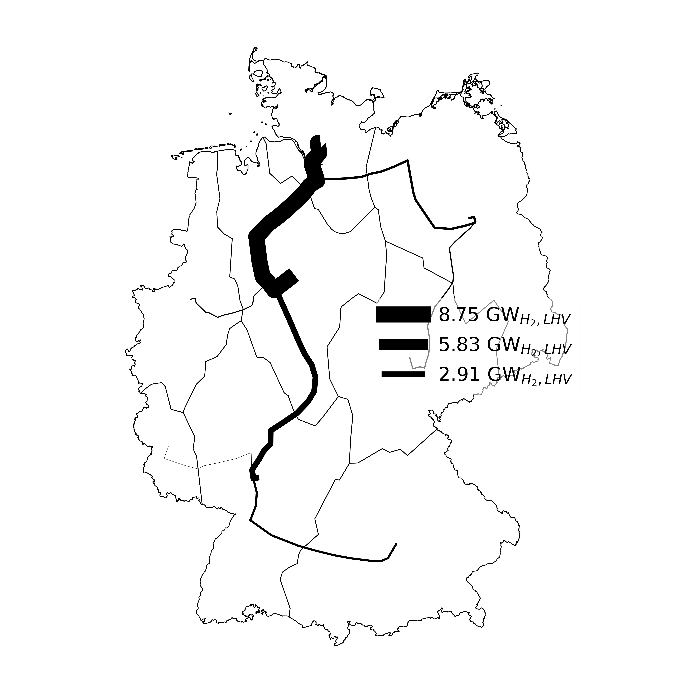
\includegraphics{images/H2Pipeline-95.png}
  \end{minipage}
  \hspace{.1\linewidth}
  \begin{minipage}[b]{.4\linewidth} 
     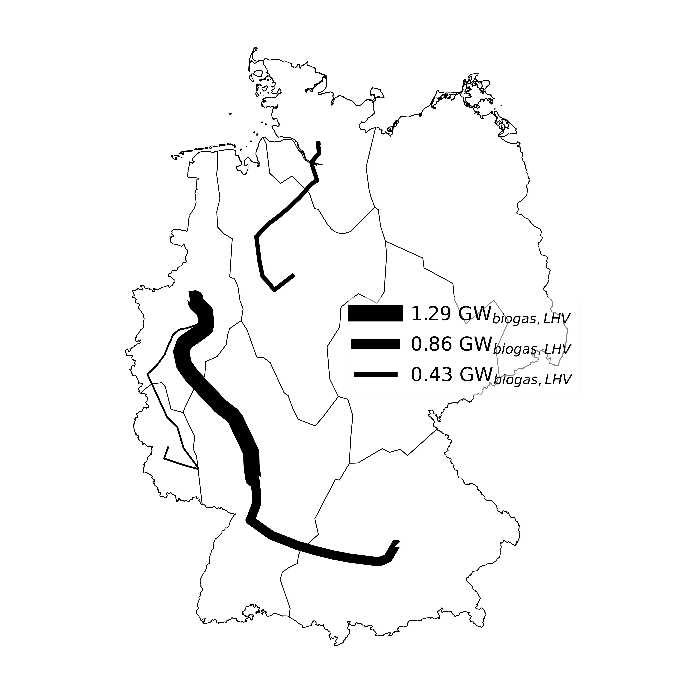
\includegraphics{images/BiogasPipeline-95.png}
  \end{minipage}
  \caption{Verläufe der Wasserstoffpipelines (links) und Biogaspipelines (rechts) der Simulation bei 95 \% CO2 Reduktion}
  \label{image:Pipelines-95}
\end{figure}

Die Grafiken in der Abbildung \ref{image:Pipelines-95} veranschaulichen die simulierten Verläufe der Wasserstoff- und Biogaspipelines. Die Wasserstoffversorgung verläuft dabei von Nord- nach Südrichtung mit großen Verbrauchern im Bereich Niedersachsens und Nordrhein-Westfalens um das Ruhrgebiet. Die Wasserstoffversorgung beginnt dabei mit ca. 8,75 GW Leistung und nimmt kontinuierlich bis zu den Endverbrauchern in Süddeutschland mit ca. 2,91 GW finaler Leistung ab. Die Versorgung mit Biogas zeigt nach Erstellung der Simulation einen getrennten Verlauf. Hierbei erstellt FINE eine kleine Versorgungstrasse mit ca. 0,43 GW installierter Leistung zwischen Schleswig-Holstein und Niedersachsen und legt die große Energieversorgung beginnend in Nordrhein-Westfalen mit 1,29 GW über Baden-Württemberg mit 0,86 GW und Bayern als Endverbraucher fest. Ein kleiner Versorgungsstrang für das Saarland und Rheinland-Pfalz wird ebenfalls simuliert.

Zum kompletten Verständnis der 95 \% Reduktion wird im Folgenden noch die zukünftige Stromversorgung in Deutschland analysiert, welche in nachfolgender Abbildung \ref{image:Leitungen-95} von FINE simuliert und visualisiert worden ist.

Das Wechselstromnetz wird dabei über alle Regionen in Nord- und Südrichtung verteilt, mit Spitzenleistungen von 18 GW elektrischer Leistung in den Haupttrassen und Verzweigungen zwischen den Knoten mit kleineren Leistungen im Bereich von ca. 12,0 GW bis 6,0 GW. Das Netz weißt dabei bereits große Ähnlichkeit mit dem heutigen Stromnetz im Jahre 2022 auf. Neu hinzugekommen sind in der Simulation die Trassen der Hochspannungsgleichstromübertragung in kurz HGÜ. Diese Technik ist relativ neu und beinhaltet insbesondere bei großen und weiten Übertragungen weniger Übertragungsverluste als Wechselstromübertragungen gleicher Größe. Hierzu können erzeugte Gleichströme von Brennstoffzellen und PV direkt in das Gleichstromnetz eingespeist und transportiert werden, wodurch eine zusätzliche Transformation in das Wechselstromnetz entfällt. Implementiert wurden diese Trassen von Fine in Nord- Süd Richtung zwischen Schleswig-Holstein und Baden-Württemberg mit einer maximalen Leistung von 4,0 GW, einer mittleren Leistung im Bereich Sachsens, Thüringen und Bayerns und einer kleinen Versorgung ausgehend von Süddeutschland in Richtung Nordrhein-Westfalens mit 1,33 GW.

\begin{figure}[!h]
  \begin{minipage}[b]{.4\linewidth} 
     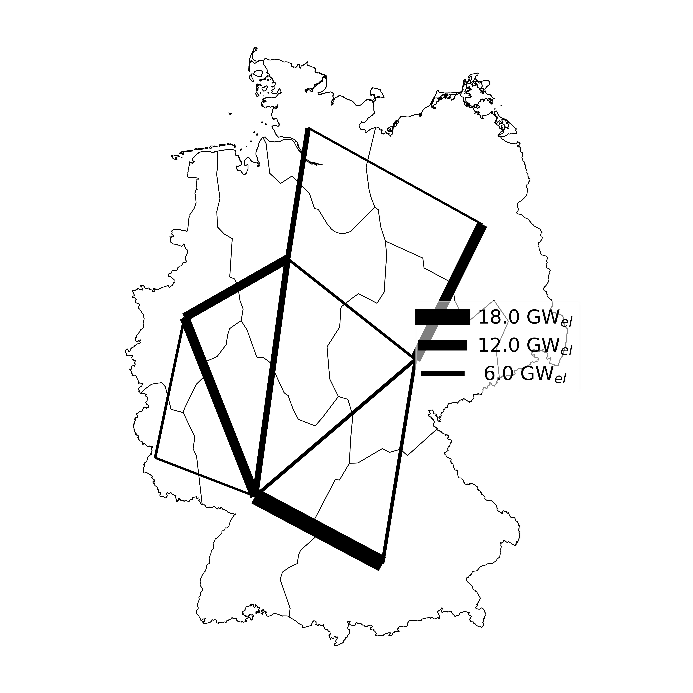
\includegraphics{images/AC-95.png}
  \end{minipage}
  \hspace{.1\linewidth}
  \begin{minipage}[b]{.4\linewidth} 
     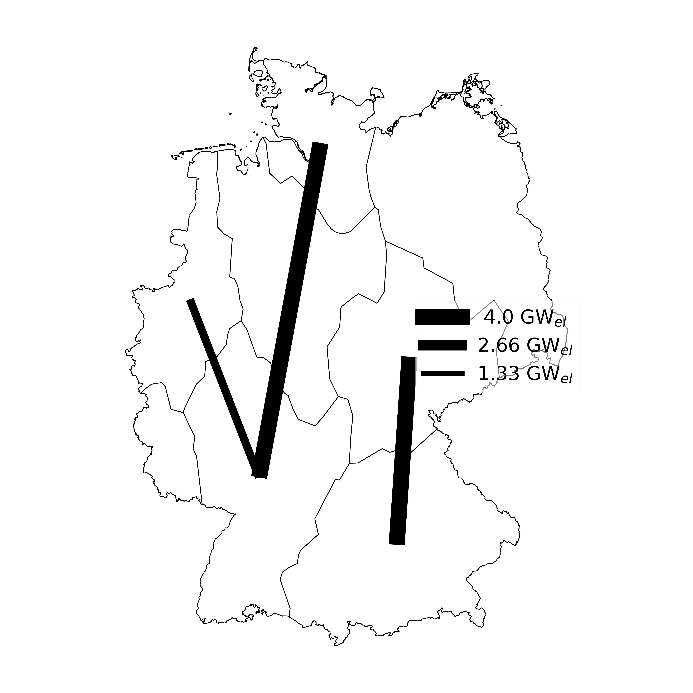
\includegraphics{images/DC-95.png}
  \end{minipage}
  \caption{Verläufe der Wechselstrom- (links) und Gleichstromtrassen (rechts) der Simulation bei 95 \% CO2 Reduktion}
  \label{image:Leitungen-95}
\end{figure}


\subsection{Reduktionsfall 100 \% (Mehdi Abbadi)}
Die Gesamtsystemkosten betragen 52 Mrd. €. Sie steigen im Vergleich zum alle Reduktionsfälle an. Insbesondere die Kosten der Wind-Offshore-Anlagen (22 Mrd. €) steigerten sich um 6 Mrd. €. Diese Steigerung wird aber teilweise durch die sinkenden Erdgas-Importe ausglichen. Hierbei verringern sich die Kosten von 15 auf 12 Mrd. €. Dies lässt sich durch die Verringerung der CO2-Emissionen erklären. Die Kosten der restlichen Erzeugungsarten sinken um etwa 2 Mrd. €.

Die Kosten der Wind-Offshore Anlagen sind massiv gestiegen im Vergleich zur Anfang Szenario (22 Mrd. €), somit steigen die Gesamtsystemkosten in höchst Szenario , betragen 52 Mrd. Dies ist ersichtlich da , die Kosten für den Gas-Import sinken . Diese Steigerung  ist auch wegen von verschiedene Speicherkapazitäten wobei die H2 Salzkavernen zum Einsatz ab dem 85 \% Fall zur Speicherung von Wasserstoff.

Die Kostenaufteilung im 100 \% Fall, nach Erzeugung, Umwandlung, Speicherung und Übertragung. Der Größte Anteil der Gesamtkosten besteht in der Erzeugung von ca. 86 \% (45 Mrd. €) als Schwerpunkt, der zweite Anteil ist durch die Speicherung zu sehen mit ca. 9 \% der Gesamten kosten (4,5 Mrd. €), danach kommen die Elektrolyse-anlagen mit ca. 2,93 Mrd. €. Die Umwandlungskosten liegen bei ca. 5,6 \% des TAC. Die restlichen 0,2 \% sind für die Übertragung geeignet.

Die gesamte installierte Leistung beträgt in allen Erzeugungsanlagen 370GW., mit einer Steigerung von ca. 50 GW zu den vorherigen Reduktionsfall. Dies kann aufgrund der massive Produktion aus der Erneuerbare Energie passieren. Da der Anteil an PV riesig angestiegen von 121 GW auf 188,2 .Die installierte Leistung an Wind-Offshore steigt  auf 81 GW als Spitzenwert, was macht lohnend bei Überschüsse, Elektrolyseanlagen nah zu den Clustern mit mehr Energie auszubauen.  Die installierte Leistung Wind-Onshore beträgt ca 44,2GW. Die Elektrolyse-Leistung steigt somit . auf den Wert maximal  23,3GW.

Bei den Batteriespeichern gibt es eine massive Steigerung. Die Speicherkapazität nimmt stark zu auf  129,46 GWh an. Dies lässt sich auf die Speicherbedarf , da die EE speisen viele Energie im Netz ein. Die Speicherung  wird dann stärker von den Batteriespeichern und von Gas Salzkavernen übernommen. Die Pumpspeicherkraftwerke haben eine deutliche geringere  Anwendung, unterscheidet sich aber nach Reduktionsfall. Dies führt dazu, dass der Einsatz von  H2- und Biogas-Salzkarvenenspeicher wichtig ist. Da deren Speicherkapazität enorme Beträge haben.
